%%%%%%%%%%%%%%%%%%%%%%%%%%%%%%%%%%%%%%%%%
% Beamer Presentation
% LaTeX Template
% Version 1.0 (10/11/12)
%
% This template has been downloaded from:
% http://www.LaTeXTemplates.com
%
% License:
% CC BY-NC-SA 3.0 (http://creativecommons.org/licenses/by-nc-sa/3.0/)
%
%%%%%%%%%%%%%%%%%%%%%%%%%%%%%%%%%%%%%%%%%
\documentclass{beamer}
\mode<presentation> {
\usetheme{Singapore}
%\usecolortheme{whale}
%\useoutertheme{shadow}
%\useoutertheme{sidebar}

%\setbeamertemplate{blocks}[rounded][shadow=true]
%\setbeamertemplate{background canvas}[vertical shading][bottom=white,top=structure.fg!25]
%\setbeamertemplate{sidebar canvas left}[horizontal shading][left=white!40!black,right=black]

}

\usepackage{graphicx} % Allows including images
\usepackage{booktabs} % Allows the use of \toprule, \midrule and \bottomrule in tables
\usepackage{listings}
\usepackage{xcolor}
\usepackage{color}
\colorlet{punct}{red!60!black}
\definecolor{background}{HTML}{EEEEEE}
\definecolor{delim}{RGB}{25,134,57}
\colorlet{numb}{magenta!60!black}

\setbeamercovered{transparent}

\usepackage{listings}
\usepackage{color}

\definecolor{dkgreen}{rgb}{0,0.6,0}
\definecolor{gray}{rgb}{0.5,0.5,0.5}
\definecolor{mauve}{rgb}{0.58,0,0.82}

\lstset{frame=tb,
  language=Java,
  aboveskip=3mm,
  belowskip=3mm,
  showstringspaces=false,
  columns=flexible,
  basicstyle={\small\ttfamily},
  numbers=none,
  numberstyle=\tiny\color{gray},
  keywordstyle=\color{blue},
  commentstyle=\color{dkgreen},
  stringstyle=\color{mauve},
  breaklines=true,
  breakatwhitespace=true,
  tabsize=3
}
%----------------------------------------------------------------------------------------
%	TITLE PAGE
%----------------------------------------------------------------------------------------
\title[@Mongoosejs]{@MongoDB + @javascript = @mongoosejs}
\author{Jesse Javier Cogollo Alvarez}
\institute[EAFIT]
{
Developer by passion \\
\medskip
\textit{twitter: @jessecogollo}
}
\date{\today}
\subject{@mongoose}

\begin{document}
	\begin{frame}
		\titlepage % Print the title page as the first slide
	\end{frame}

	\begin{frame}
		\frametitle{Contenido}
		\tableofcontents
	\end{frame}

%----------------------------------------------------------------------------------------
%	PRESENTATION SLIDES
%----------------------------------------------------------------------------------------

%\begin{frame}
%\frametitle{Some background}
%We start our discussion with some concepts.
%\pause
%The first concept we introduce originates with Erd\H os.
%\pause
%otro pause
%\pause
%mas pausse...
%\pause
%\end{frame}

%\begin{frame}
%	\frametitle{`Hidden higher-order concepts?'}
%	\begin{itemize}[<+->]
%	\item The truths of arithmetic which are independent of PA in some 
%	sense themselves `{contain} essentially {\color{blue}{hidden higher-order}},
%	 or infinitary, concepts'???
%	\item `Truths in the language of arithmetic which \ldots
%	\item	That suggests stronger version of Isaacson's thesis. 
%	\end{itemize}
%\end{frame}
%------------------------------------------------
\section{MongoDB}
%------------------------------------------------
\begin{frame}
\frametitle{Que es @MongoDB}
'MongoDB (from "humongous") is an open-source document database, and the leading NoSQL database. Written in C++.'
{\color{blue}\url{https://www.mongodb.org/}}
\pause
\\~\\
'MongoDB was not designed in a lab. We built MongoDB from our own experiences building large-scale,high availability, robust systems...'
\underline{\color{green}Eliot Horowitz, CTO and Co-Founder}	
\end{frame}
%------------------------------------------------
\begin{frame}
\frametitle{NOSQL}
“En inform\'atica, NoSQL (a veces llamado 'no só\'olo SQL') es una amplia clase de sistemas de gesti\'on de bases de datos que difieren del modelo cl\'asico del sistema de gesti\'on de bases de datos relacionales (RDBMS) en aspectos importantes, el m\'as destacado que no usan SQL como el principal lenguaje de consultas.” {\color{blue}\url{http://es.wikipedia.org/wiki/NoSQL/}}
\\~\\
\end{frame}
%------------------------------------------------

\begin{frame}
\frametitle{NOSQL}
Las caracteristicas comunes de las bases de datos NoSQL son:
\begin{itemize}[<+->]
\item No utilizan el modelo relacional.
\item Corren bien en clusters.
\item Open-source.
\item sin esquemas.
\item El resultado mas importante del aumento de las bases de datos NoSQL es la {\color{green}Persistencia Pol\'iglota}.
\\~\\
{\color{blue}\url{http://martinfowler.com/articles/nosqlKeyPoints.html}}
\end{itemize}

\end{frame}

%------------------------------------------------
\begin{frame}
\frametitle{Persistencia pol\'iglota}
\begin{figure}
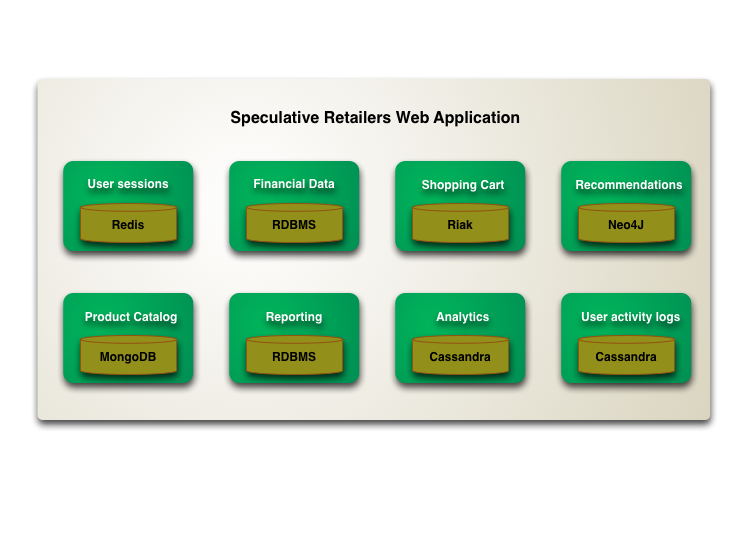
\includegraphics[width=1.0\linewidth]{polyglot.png}
\end{figure}
\end{frame}

%------------------------------------------------
\begin{frame}
\frametitle{Caracteristicas}
\begin{columns}[c]

\column{.45\textwidth} % Left column and width
\begin{enumerate}
\pause
\item Document-Oriented Storage
\pause
\item Full Index Support
\pause
\item Replication
\pause
\item Auto Sharding
\pause
\item Querying
\pause
\item Map Reduce
\pause
\item GridFS
\pause
\item \textbf{Other more...}
\end{enumerate}
\column{.5\textwidth} % Right column and width
\begin{itemize}
\item MMS.
\item Partner with MongoDB.
\item Multiples drivers.
\end{itemize}
\end{columns}
\end{frame}

%------------------------------------------------
\begin{frame}
\frametitle{Insert Find Update Remove (CRUD)}
\begin{block}{\textbf{I}FUR}
db.meetups.insert(\{"name":"mongoosejs","place":"Ruta N"\})
\end{block}
\begin{block}{I\textbf{F}UR}
db.meetups.find(\{"name":"mongoosejs"\})
\end{block}
\begin{block}{IF\textbf{U}R}
db.meetups.update(\{"name":"mongoosejs"\},
\{\$set:\{"description":"Ruta N, piso 0."\}\})
\end{block}
\begin{block}{IFU\textbf{R}}
db.meetups.remove(\{"name":"mongoosejs"\})
\end{block}
\end{frame}

%------------------------------------------------
\section{javascript}
%------------------------------------------------
\begin{frame}
\frametitle{NodeJS - IOJS}
NodeJS es una plataforma de javascript construida sobre el "motor" V8 de Chrome.
{\color{blue}\url{https://nodejs.org//}}
\pause
\\~\\
IOJS es un fork de NodeJS. Implementando ES6 y desarrollado bajo un modelo de gobierno abierto.
{\color{blue}\url{https://iojs.org//}}
\end{frame}
%------------------------------------------------	
\section{mongoose}
\begin{frame}
\frametitle{mongoose}
\pause
instalaci\'on
\\~\\
\end{frame}

\begin{frame}[fragile]
\frametitle{Inserting source code}
\lstset{language=C++,
                basicstyle=\ttfamily,
                keywordstyle=\color{blue}\ttfamily,
                stringstyle=\color{red}\ttfamily,
                commentstyle=\color{green}\ttfamily,
                morecomment=[l][\color{magenta}]{\#}
}
\begin{lstlisting}
    #include<stdio.h>
    #include<iostream>
    // A comment
    int main(void)
    {
    printf("Hello World\n");
    return 0;
    }
\end{lstlisting}
\end{frame}

\begin{frame}[fragile]
\frametitle{Inserting source code without setting typewriter}
\lstset{language=C++,
                keywordstyle=\color{blue},
                stringstyle=\color{red},
                commentstyle=\color{green},
                morecomment=[l][\color{magenta}]{\#}
}
\begin{lstlisting}
    #include<stdio.h>
    #include<iostream>
    // A comment
    int main(void)
    {
    printf("Hello World\n");
    return 0;
    }
\end{lstlisting}
\end{frame}

\defverbatim[colored]\lstI{
\begin{lstlisting}[language=C++,basicstyle=\ttfamily,keywordstyle=\color{red}]
int main() {
  // Define variables at the beginning
  // of the block, as in C:
  CStash intStash, stringStash;
  int i;
  char* cp;
  ifstream in;
  string line;
[...]
\end{lstlisting}
}

\begin{frame}{A Listings Demo}{C++}
\lstI
\end{frame}


\begin{frame}[fragile]
\begin{lstlisting}
// Hello.java
import javax.swing.JApplet;
import java.awt.Graphics;

public class Hello extends JApplet {
    public void paintComponent(Graphics g) {
        g.drawString("Hello, world!", 65, 95);
    }    
}
\end{lstlisting}
\end{frame}

\begin{frame}[fragile]

\newcommand{\shellcmd}[1]{\\\indent\indent\texttt{\footnotesize\# #1}\\}
  \noindent Consider the following command:
  \shellcmd{apt-get --purge remove rubygems}
  This removes the \texttt{rubygems} package.

\end{frame}

\begin{frame}
\frametitle{Comunidad}
\begin{enumerate}
\item Meetup: medellinjs  - mongodbmedellin
\pause
\item Twitter: @medellinjs - @mongodbmedelln
\pause
\item Facebook: /mongodbmedellin
\pause
\item gitter (chat): https://gitter.im/coljs/medellinjs
\pause
\item gitter (chat): https://gitter.im/MongoDBMedellin/Meetup
\end{enumerate}
\end{frame}
%------------------------------------------------	
\begin{frame}
\frametitle{Donde aprender}
\footnotesize{
\begin{thebibliography}{99} % Beamer does not support BibTeX so references must be inserted manually as below
\bibitem[]{p1} javascript (nodeJS)
\newblock http://nodeschool.io//
\end{thebibliography}
}

\footnotesize{
\begin{thebibliography}{99} % Beamer does not support BibTeX so references must be inserted manually as below
\bibitem[]{p1} MongoDB
\newblock https://university.mongodb.com/
\end{thebibliography}
}
\end{frame}

%------------------------------------------------
\begin{frame}
\frametitle{Preguntas}
\end{frame}

%------------------------------------------------
\begin{frame}
\Huge{\centerline{Gracias !!! =)}}
\end{frame}
%----------------------------------------------------------------------------------------

\end{document} 
